% Backup — Heatmap CTI/BE/NS por política e POD simplificado (figura isolada)
\begin{frame}[noframenumbering]{[Backup] CTI, efeito \textit{bullwhip} e NS por política e perfil}
  \centering
  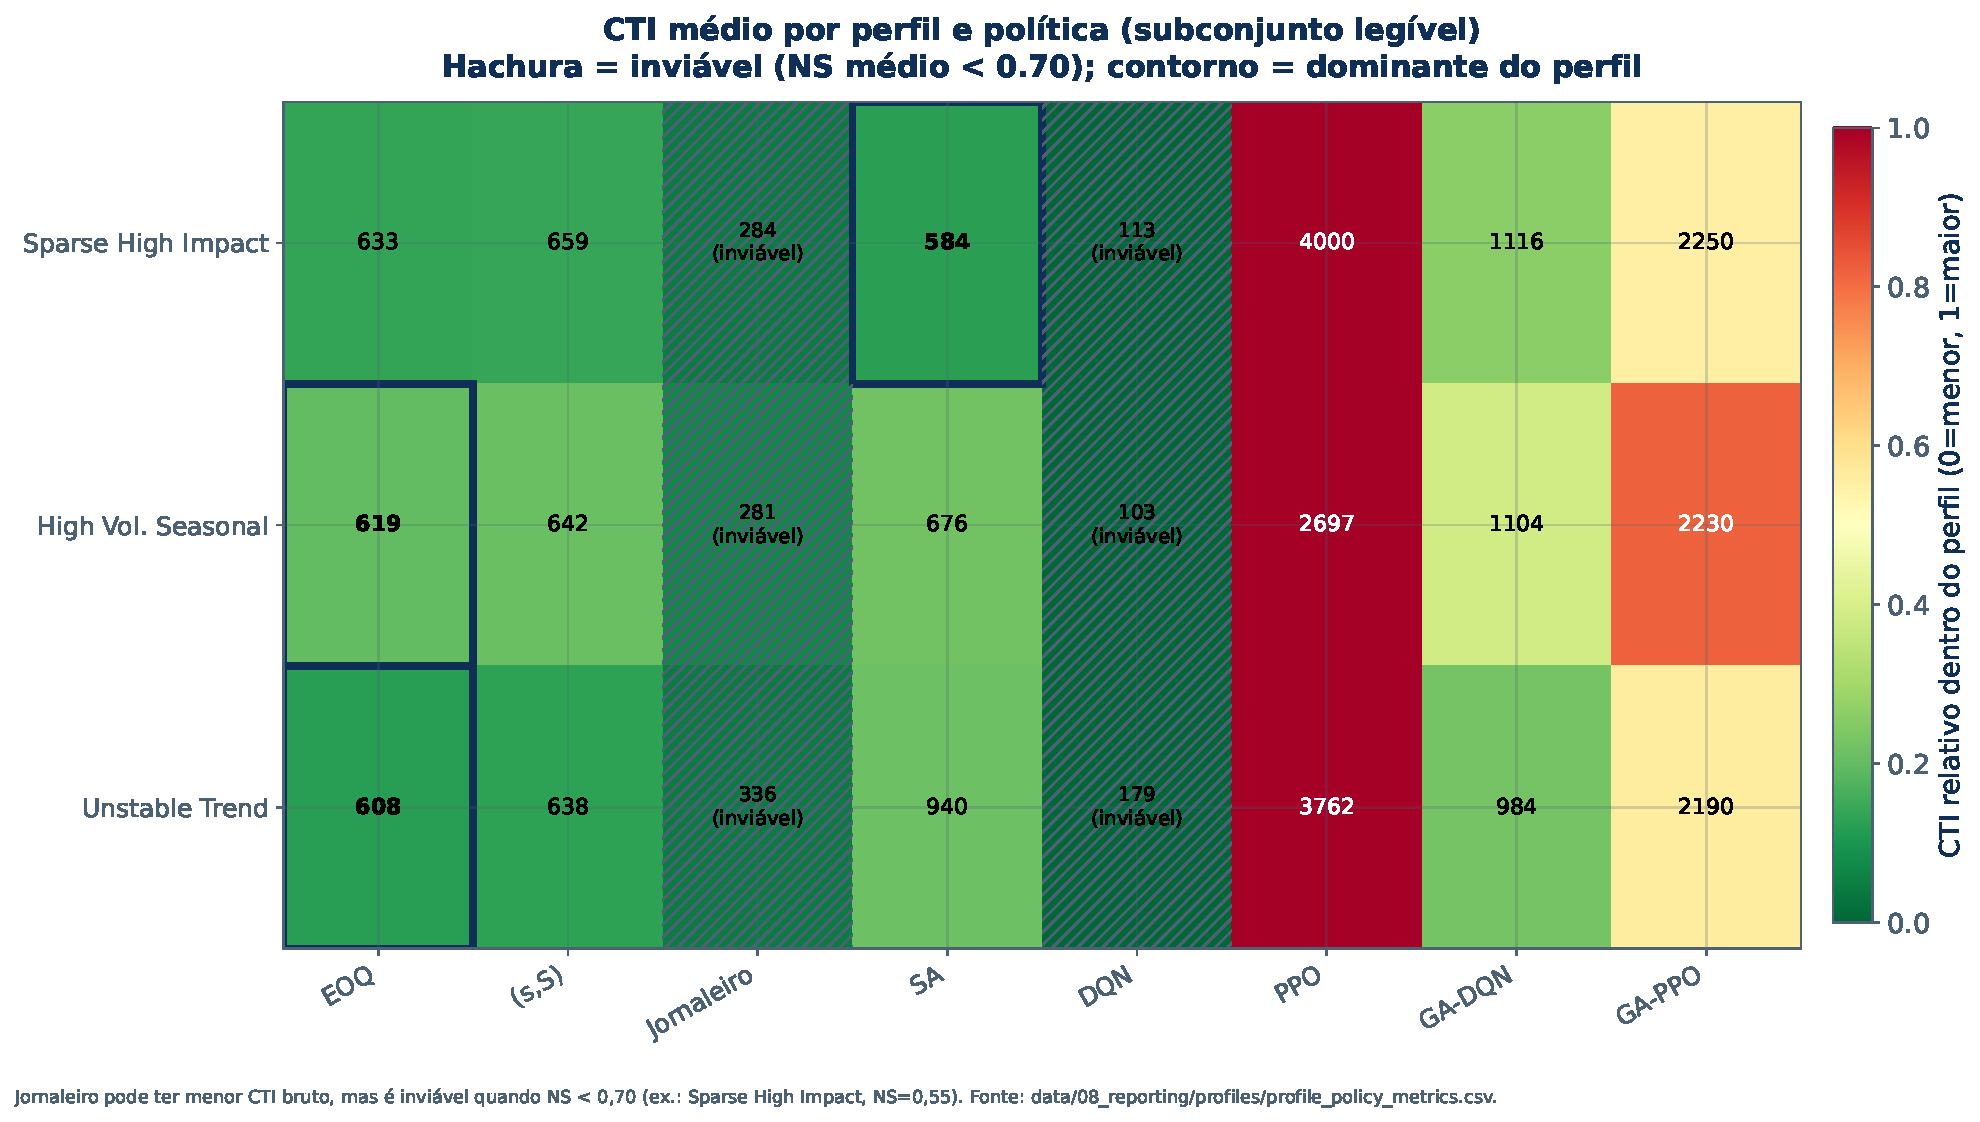
\includegraphics[width=0.88\linewidth,height=7.0cm,keepaspectratio]{figures/profile_policy_heatmap_simplified.pdf}
  \note{
    Esta versão simplificada do heatmap restringe a um subconjunto legível
    de políticas, mantendo sempre a política viável de menor CTI de cada
    perfil (contorno em destaque) e marcando com hachura as combinações
    inviáveis, com NS médio abaixo de 0,70 -- caso do Jornaleiro e do DQN.
    Cada célula agora mostra três indicadores: o CTI médio, o BE médio
    (efeito \textit{bullwhip}, Var(Q)/Var(D)) e o NS médio daquela política
    naquele perfil -- por exemplo, a SA domina em Sparse High Impact não só
    pelo menor CTI entre as viáveis, mas também com BE baixo (6,2) e NS de
    0,86, enquanto o Jornaleiro, hachurado, mostra exatamente por que é
    inviável: NS de 0,55, visível na própria célula. O ponto central
    continua o mesmo do heatmap completo: a mesma política produz custo,
    estabilidade e serviço muito distintos segundo o perfil, e nenhuma
    política os otimiza simultaneamente em todos os perfis. Essa
    heterogeneidade é a evidência visual direta que motiva a seleção
    contextual por perfil.
  }
\end{frame}
